\documentclass[12pt,letterpaper]{report}
\usepackage[utf8x]{inputenc}
\usepackage{ucs}
\usepackage{graphicx}
\usepackage{url}
\author{Zi Yan, Xin Jin, Bo Tang}
\title{TCP/IP Packet Assembler \& Analyzer Final Report}
\date{}
\begin{document}
\maketitle

\chapter*{Project Description}
Write a software that can send packets to target system using 
user specified parameters and receive and analyze the respond. 
The software should be designed like an API to make it easier 
to use this software in other applications. The software should 
be able to provide the following functionalities.

\begin{itemize}
 \item Support TCP protocol
 \item Support ICMP protocol
 \item Support UDP protocol
\end{itemize}

\chapter*{Related Materials}
\section*{Protocols}
TCP/IP stands for Transmission Control Protocol/Internet Protocol. 
TCP/IP is the communication protocol for communication between 
computers on the Internet. TCP/IP defines how electronic devices 
(like computers) should be connected to the Internet, and how 
data should be transmitted between them.

Inside the TCP/IP standard there are several protocols for 
handling data communication:

\begin{itemize}
 \item TCP (Transmission Control Protocol) communication between
  applications,the content in TCP packet can be seen in Figure \ref{tcpheader}
  \cite{1}. 
 \item UDP (User Datagram Protocol) simple communication between 
 applications, the content in UDP header can be seen in Figure \ref{udpheader}
 \cite{2}.
 \item IP (Internet Protocol) communication between computers, the content in IP packet can be seen in Figure \ref{ipheader}\cite{3}.
 \item ICMP (Internet Control Message Protocol) for errors and 
 statistics. Generally, there are 6 ICMP packet types which are 
 icmp\_echo, icmp\_unreach, icmp\_timeexceed, icmp\_timestamp, 
 icmp\_mask and icmp\_redirect. There are also some subtypes 
 of these general type. For example, icmp\_echo type can be 
 separated in 2 subtypes: icmp\_echo\_request and icmp\_echo\_reply. 
 Each of the types and subtypes has destined type number. 
 The content in header can be seen in Figure \ref{icmpheader}\cite{4}.
\end{itemize}

\begin{figure}[!htp]
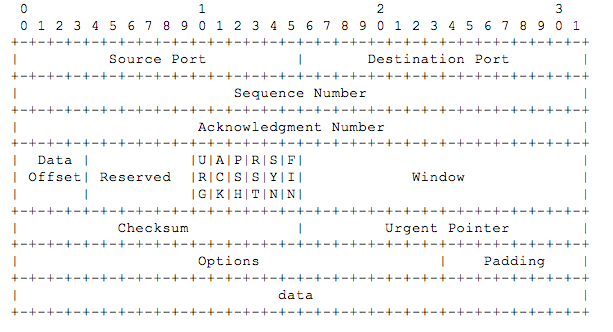
\includegraphics[width=\linewidth]{figure1.png}
\caption{TCP Header Format}
\label{tcpheader}
\end{figure}

\begin{figure}[!htp]
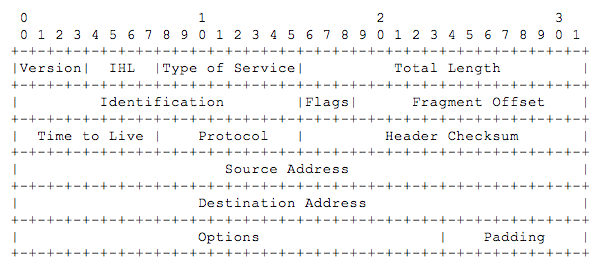
\includegraphics[width=\linewidth]{figure2.png}
\caption{Example Internet Datagram Header}
\label{ipheader}
\end{figure}

\begin{figure}[!htp]
\centering
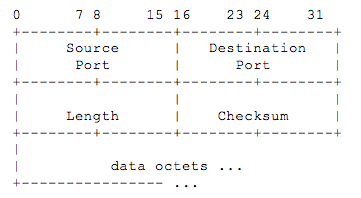
\includegraphics[width=0.5\linewidth]{figure3.png}
\caption{User Datagram Header Format}
\label{udpheader}
\end{figure}

\begin{figure}[!htp]
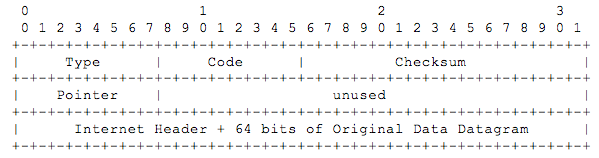
\includegraphics[width=\linewidth]{figure4.png}
\caption{Internet Control Message Protocol Header Format}
\label{icmpheader}
\end{figure}

\section*{Libnet, Tcpdump and Wireshark}
Libnet is a generic networking API that provides access to 
several protocols. It is not designed as a 'all in one' solution 
to networking \cite{5}. In our project, we generally use the 
libnet APIs to initialize the network, construct packet and 
inject the packet.

Tcpdump is a common packet analyzer that runs under the 
command line. It allows the user to intercept and display 
TCP/IP and other packets being transmitted or received 
over a network to which the computer is attached\cite{6}. 
We need to run the tcpdump as super user and use 
proper flags to print the response. 

We also use wireshark\cite{7} when we are simulating IP 
spoof  by forging source IP address when sending ICMP 
packet. Wireshark is the world's foremost network protocol 
analyzer. It lets you capture and interactively browse the 
traffic running on a computer network. It is the de facto 
(and often de jure) standard across many industries and 
educational institutions.

\chapter*{Design}

\section*{User Interface}
Considering that the program will be cross-platform, we 
are planning to adopt a GUI which can be used under all
three mainstream OS, Windows, Mac OS, and Linux.

First, we considered Qt and GTK, but both of them involve
large libraries which are cumbersome to use for such a
small program. Therefore, we choose to use a web page
as our GUI. Without any additional compilation, a web page
can be accessed in any OS.

We use a web page to get the user parameter and send all 
the packets to server where our main program is located.
 In this interface, we have three options for the type of 
 packet and for each type the user has chosen, he need 
 to set parameter for each required field and send the 
 request after finished.
 
 \section*{Using Libnet}
 After we get the parameters, we send the request to 
 our server where our main program is located. We use 
 the functions in Libnet to finish sending the packet. 
 First we need to initialize the network using 
 
 \textit{ libnet\_init( LIBNET\_RAW4,NULL, err\_buf);}
 
 and then build each packet using API in Libnet. For 
 example, we use the following function to build UDP 
 header:
 
 \textit{libnet\_ptag\_t libnet\_build\_udp(u\_int16\_t  sp, 
 u\_int16\_t  dp, u\_int16\_t  len, u\_int16\_t  sum, u\_int8\_t*  
 payload, u\_int32\_t  payload\_s, libnet\_t*  l, libnet\_ptag\_t  
 ptag  );}
 
 And then we build the IP header using the following function:
 
 \textit{libnet\_ptag\_t libnet\_build\_ipv4(u\_int16\_t  ip\_len, 
 u\_int8\_t  tos, u\_int16\_t  id, u\_int16\_t  frag, u\_int8\_t  ttl, 
 u\_int8\_t  prot, u\_int16\_t  sum, u\_int32\_t  src, u\_int32\_t  dst,
  u\_int8\_t*  payload, u\_int32\_t  payload\_s, libnet\_t*  l, 
  libnet\_ptag\_t  ptag  );}
 
Afterwards, we inject the packet into destination address and 
port using the following function:

\textit{libnet\_write(network);}

And use this function to close the network:

\textit{libnet\_destroy(network);}

\section*{Encapsulation of functions and parameters}
We write three classes which encapsulate the operation and 
parameter for each packet. 

In general, for each packet, all of them have network 
initialization, its own header construction, IP layer construction,
sending the constructed packet, and freeing the memory. The 
only difference is that different protocols will need different 
parameters and use different ``build" functions. So we use 
different parameter setter functions, and manipulate corresponding
``build" functions for each protocols.


\section*{Using Tcpdump and Wireshark to capture packets}
For Tcpdump, the commands we use are referred to following
template:

\textit{sudo tcpdump -A -vv -i \textless interface\textgreater dst 
\textless dst ip \textgreater and port \textless dst port \textgreater}

\chapter*{Implementation}
The structure of the program is constructed by Zi Yan, and 
Zi Yan finishes UDP and HTTP server, Bo Tang finishes ICMP, 
Xin Jin finishes TCP and we together connect and debug the 
user interface and main program. 

\section*{User Interface}
We write a simple interface where user can construct packet 
and send packet. The screen shot is shown in Figure \ref{ui}:

\begin{figure}[!htp]
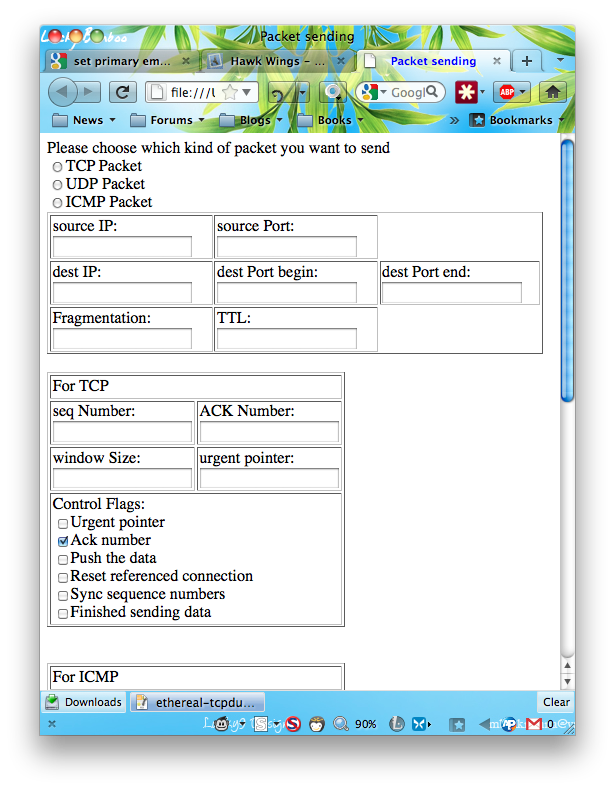
\includegraphics[width=0.5\linewidth]{ui1.png}
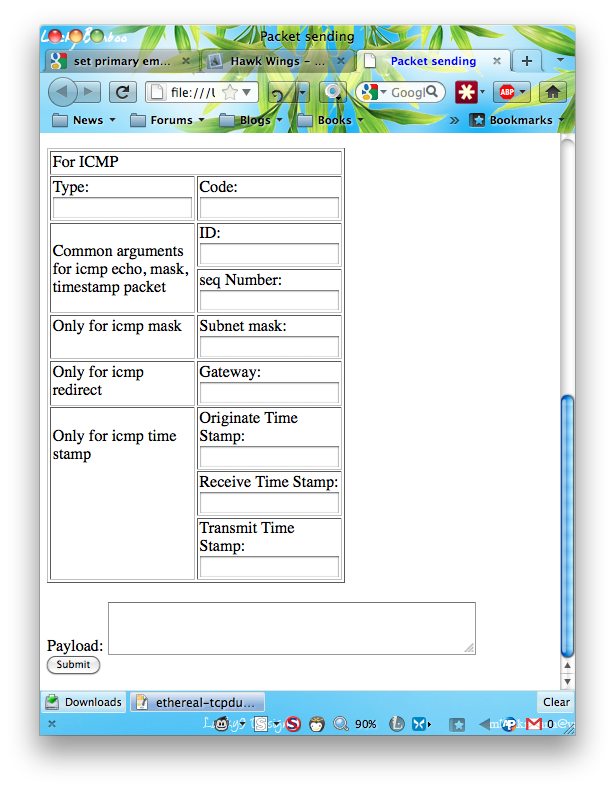
\includegraphics[width=0.5\linewidth]{ui2.png}
\caption{User Interface}
\label{ui}
\end{figure}


\section*{Back End}
As we said in design part, after we get the parameters 
from user, we use API to construct packet and send packet. 
Due to the length of this report, we omit our code 
implementation.

Generally, a function-limited HTTP server is running 
at the back end, receiving HTTP request from the 
browser at a certain port, either assigned by user or 
set to 3333 in default. Only GET and POST methods
will be processed. After a request from the browser
is received, the server will interpret the HTTP request
and invoke corresponding classes, either TCP, UDP, or
ICMP. After sending a packet, a message, either 
success or failure, will be sent back to the browser
to tell the user the result. 

\chapter*{Experimental Analysis}
\section*{Sending TCP packets}
The configuration is as follows:
\begin{itemize}
 \item Actual ending Machine: 129.115.30.201 and forged 
 source IP is: 129.115.30.204,
 \item Destination Machine: 129.115.102.107,
 \item Receive Machine:129.115.30.204 which is the forged 
 source IP address.
\end{itemize}

We use the machine 129.115.30.201 to send the packet 
to make TCP connect with machine 129.115.102.107. We 
forged an source IP address as 129.115.30.204 and then 
send the packet, it can be seen in Figure \ref{tcp1}. We noticed that 
the destination machine keep on sending several packet 
containing <ack,seq> message to the forged machine to 
try to respond to the connection, and we can see it in 
Figure \ref{tcp2}.

\begin{figure}[!htp]
\centering
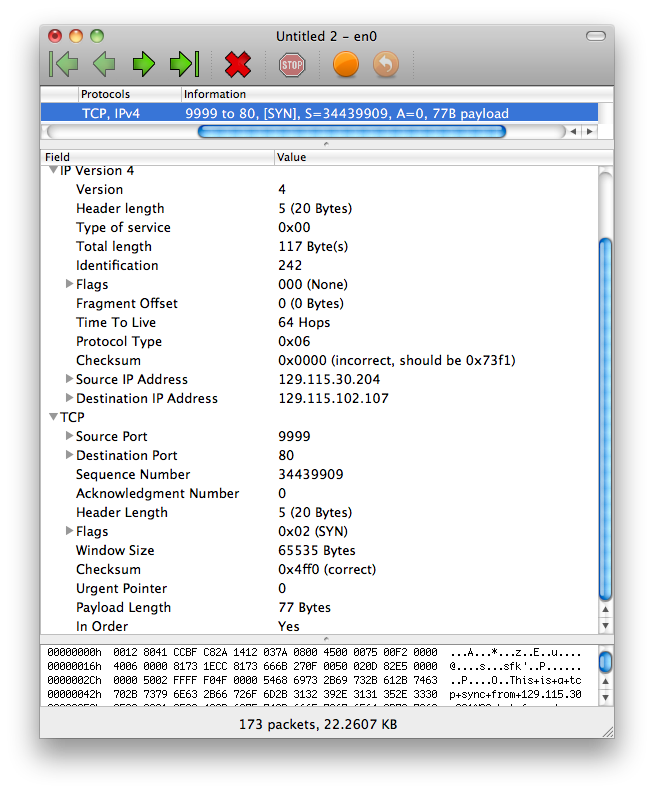
\includegraphics[width=0.8\linewidth]{tcp1.png}
\caption{Sending a TCP packet}
\label{tcp1}
\end{figure}


\begin{figure}[!htp]
\centering
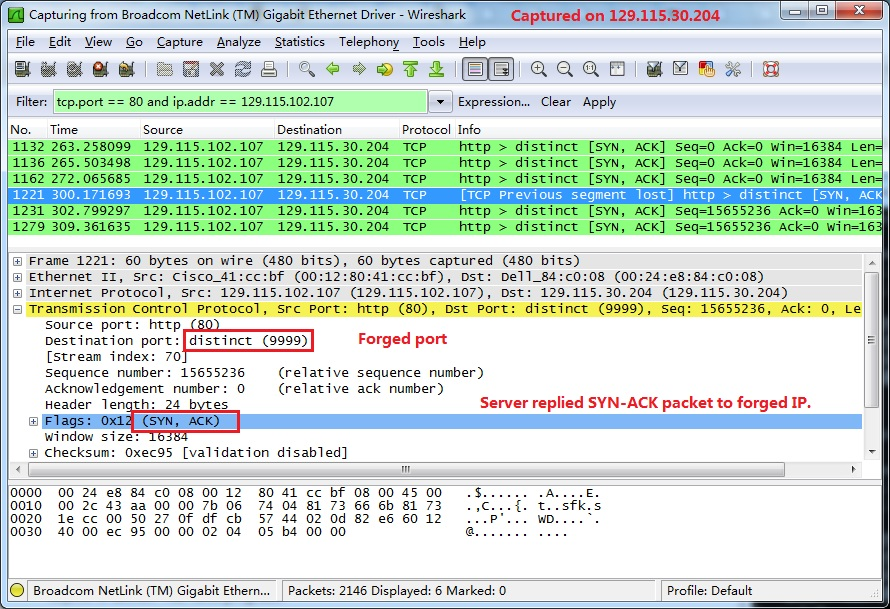
\includegraphics[width=\linewidth]{tcp2.jpg}
\caption{Receiving a TCP packet}
\label{tcp2}
\end{figure}

\section*{Sending UDP packets}
The configuration is as follows:
\begin{itemize}
 \item Actual Source IP: 129.115.30.201, Forged Sourced 
 IP: 129.115.30.204,
 \item Destination IP:129.115.30.204.
\end{itemize}

We build a UDP packet and set the source IP as the same as 
the destination IP and send the packet to destination machine, 
it can be seen from Figure \ref{udp1}. On destination machine, we 
can detect the packet as the same as sent, and this is shown
in Figure \ref{udp2}.

\begin{figure}[!htp]
\centering
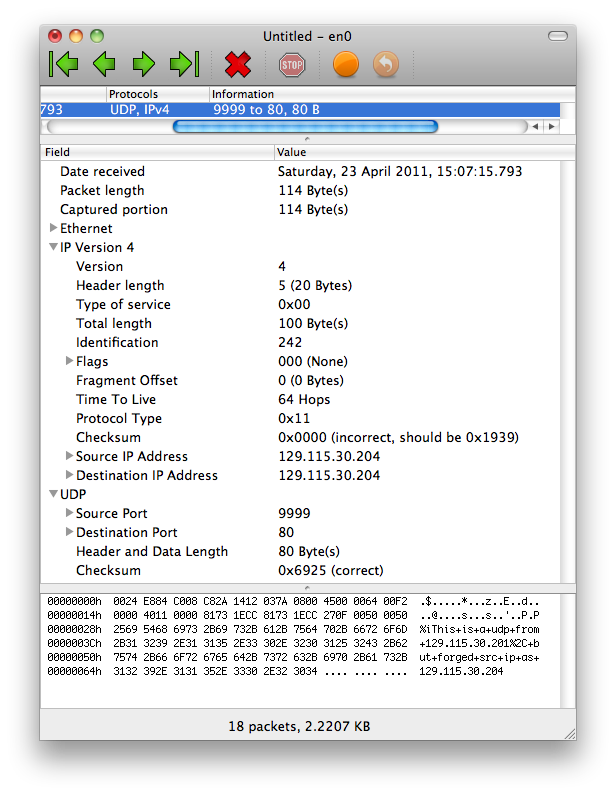
\includegraphics[width=0.8\linewidth]{udp1.png}
\caption{Sending a UDP packet}
\label{udp1}
\end{figure}


\begin{figure}[!htp]
\centering
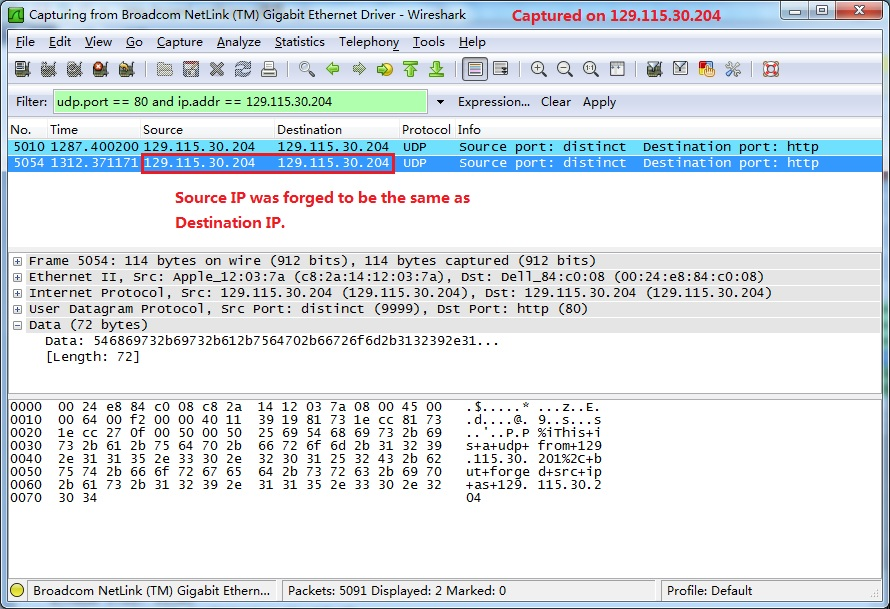
\includegraphics[width=\linewidth]{udp2.jpg}
\caption{Receiving a UDP packet}
\label{udp2}
\end{figure}

\section*{Sending ICMP packets}
We send a ICMP\_ECHO\_REQUEST message to the gateway 
and forge the source, it can be seen from Figures \ref{icmp1}. So 
the gateway return a ICMP\_ECHO\_REPLY message to the 
forged machine, where it is shown in Figure \ref{icmp2}.

\begin{figure}[!htp]
\centering
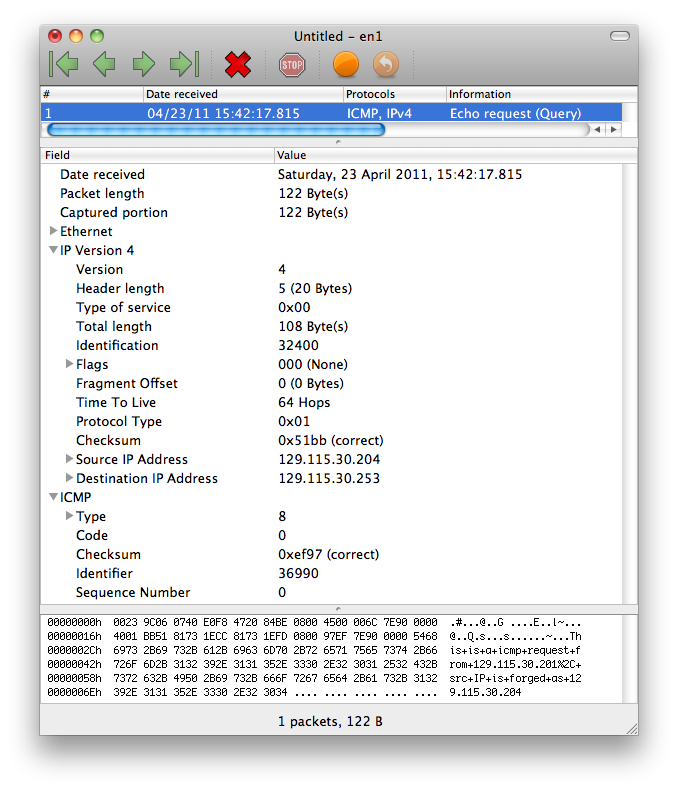
\includegraphics[width=0.8\linewidth]{icmp1.png}
\caption{Sending a ICMP packet}
\label{icmp1}
\end{figure}


\begin{figure}[!htp]
\centering
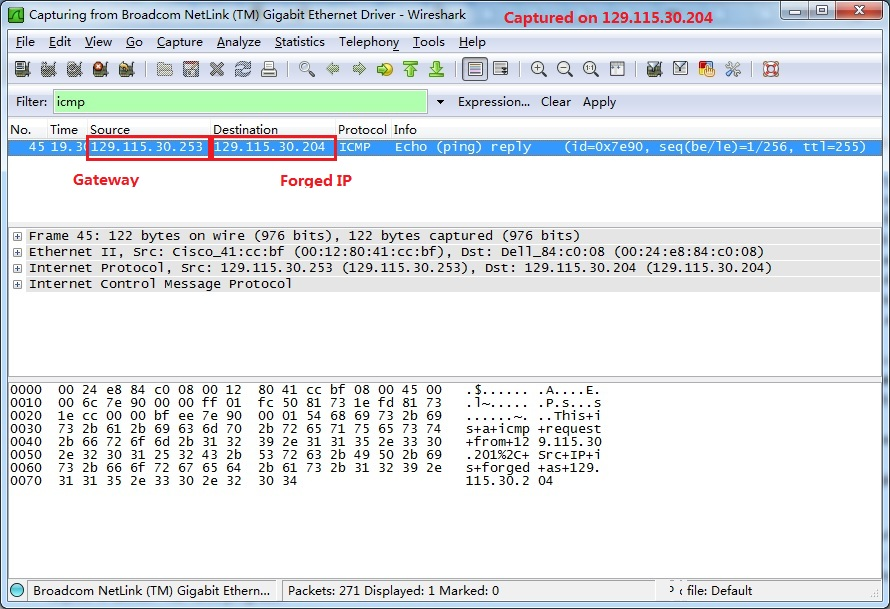
\includegraphics[width=\linewidth]{icmp2.jpg}
\caption{Receiving a ICMP packet}
\label{icmp2}
\end{figure}



\chapter*{Conclusion}
In this project, we have designed and implemented a packet 
construction tool. It supports TCP, UDP and ICMP transportation 
level protocols. There is also a webpage based user interface 
which connects to the back end program.

With this tool, users are able to construct and send packets 
with arbitrary parameters in all of the three protocols. We 
have also experimented with several hacking approaches 
such as TCP half-open attacks, SYN-Flood attacks, ICMP 
and UDP spoof attacks and reflection attacks, etc. Some of 
the attack behaviors are obvious with packet sniffer tools, 
such as Wireshark and tcpdump. Future work can be done 
in implementing batch processing tools which can be 
utilized in controlled flooding attacks or DDoS attacks.

\bibliographystyle{plain}
\bibliography{finalreport}
\end{document}